\begin{bclogo}[couleur = gray!20, arrondi = 0.2, logo=\bcattention]{Incremental code}
As for the last two sessions, we provide you with a "golden version" of the project at this point. If you are not sure about the correctness of your implementation, download \texttt{p2c.patch} from Moodle and apply it to your repository. Note that the patches are incremental, meaning that you must apply \texttt{p2a.patch} and \texttt{p2b.patch} (if not already done), then \texttt{p2c.patch} on top of it.
\end{bclogo}

\section{Packetizing the feature vector}

\subsection{Filling in the packet header}

In our application, a packet is composed of the \textbf{header} containing multiple fields, the \textbf{payload} which is the actual feature vector and the \textbf{tag} for authentication. Open the files \texttt{transfer.c}/\texttt{.h}. The implementation of the function \texttt{make\_packet()} is incomplete, follow the instructions in \textbf{the first step} of that function to fill in the header. \textit{Hint:} Check out the variables defined in \texttt{transfer.c} and the macros in \texttt{transfer.h}. Take care of the endianness for multi-byte fields.

\begin{bclogo}[couleur = gray!20, arrondi = 0.2, logo=\bcinfo]{Endianness}
	When dealing with multi-byte data (e.g. \texttt{uint16\_t} or \texttt{uint32\_t}, but not \texttt{uint8\_t} that is 1-byte long), there are two main ways of ordering the individual bytes inside the larger group :
	\begin{itemize}
		\item \textbf{Big-endian (BE)} stores the \textit{most} significant bytes first (i.e. at the smallest memory address);
		\item \textbf{Little-endian (LE)} stores the \textit{least} significant bytes first, or equivalently the most significant bytes last.
	\end{itemize}
    Take for example a 32-bit unsigned integer $x \in \{0,\dots, 2^{32}-1\}$.
    Let $x_0,x_1,x_2,x_3\in\{0,...,255\}$ be such that $x = \sum_{i=0}^3 x_i 256^i$.
    The BE encoding of $x$ is
    \texttt{$x_3$$\mathbin\Vert$$x_2$$\mathbin\Vert$$x_1$$\mathbin\Vert$$x_0$}
    while its LE encoding is
    \texttt{$x_0$$\mathbin\Vert$$x_1$$\mathbin\Vert$$x_2$$\mathbin\Vert$$x_3$},
    with $\mathbin\Vert$ denoting the \textit{concatenation}.
\end{bclogo}

Notice that the second step in \texttt{make\_packet()} is already implemented : each mel value of each mel-vector is copied from the computed array to the packet structure.

\subsection{Generating an authentication tag}

Let us now consider the authentication of the packet. The authentication \texttt{tag} is defined as
\[
    \texttt{tag} = \text{CBC-MAC-AES}_{k}\left(
        \texttt{header$\mathbin\Vert$payload}
    \right)\;,
\]
where $k$ is a secret key (a sequence of 16 uniformly random bytes) shared between the MCU and the receiver. The $\text{CBC-MAC-AES}$ algorithm is described in \autoref{algo:cbc-mac-aes} and its block diagram is shown in \autoref{fig:cbc-mac-aes}.

Complete the third step of \texttt{make\_packet()} by implementing the algorithm with the following constraints: the function \textbf{must not allocate memory}, and its stack space usage must be constant (i.e., independent of the message length).
We provide you with the AES reference implementation (\texttt{aes\_ref.h} in \textbf{Drivers/AES/}), whose
prototype is the following:
\begin{lstlisting}[style=customc]
void AES128_encrypt(unsigned char* block, const unsigned char* key);
\end{lstlisting}
where \texttt{block} is both the input and output of the AES block cipher (it
is modified in-place).
Both \texttt{block} and \texttt{key} are expected to point to 16-byte buffers. Regarding the key, you can modify and use the \texttt{AES\_Key} variable defined on top of the file.

\begin{algorithm}
\begin{algorithmic}
    \REQUIRE Message $x$ (sequence of bytes) to authenticate.
    \REQUIRE Secret key $k$ (sequence of 16 bytes)
    \ENSURE The authentication tag $t$ (sequence of 16 bytes).
    \STATE Parse $x$ into blocks $\left(x_1,x_2,\dots,x_n\right)$ such that the
    length of each block is 16 bytes (except for $x_n$).
    \STATE If the length of $x_n$ is not 16, append as many zero bytes to $x_n$
    to extend it to 16 bytes.
    \STATE $state \leftarrow 0^{16}$ (Where $0^{16}$ denotes the string made of 16 zero bytes.)
    \FOR{$i=1\dots,n$}
    \STATE $state \leftarrow \text{AES}_k(state \oplus x_i)$
    \ENDFOR
    \STATE $tag \leftarrow state$
\end{algorithmic}
\caption{CBC-MAC-AES}
\label{algo:cbc-mac-aes}
\end{algorithm}

\begin{figure}[h]
\centering
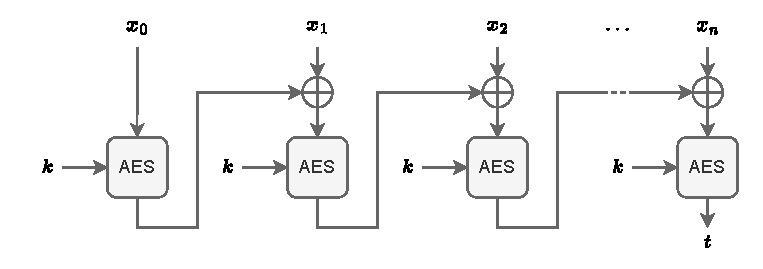
\includegraphics[scale=1]{figures/crypto_cbc_mac_aes.pdf}
\caption{Block diagram of CBC-MAC-AES}
\label{fig:cbc-mac-aes}
\end{figure}

\begin{bclogo}[couleur = gray!20, arrondi = 0.2, logo=\bcquestion]{Header and tag}
\begin{itemize}
	\item What is the use of each field of the header ? 
	\item You have had a quick introduction to the authentication basic knowledge in Lecture L2b. Based on that and on the description of the message authentication code, what is your understanding of the purpose of the authentication tag ? What kind of attacks does it prevent ? More importantly, what \textit{doesn't} it prevent ? Is the header readable or encrypted ? And the payload ?
\end{itemize}
\end{bclogo}

Once you have correctly implemented the function \texttt{make\_packet()}, open the file \texttt{main.c} and replace the call to \texttt{print\_melvectors()} by two function calls : 
\begin{itemize}
	\item \texttt{make\_packet()}, you just implemented it;
	\item then \texttt{send\_packet()} that either prints the formatted packet via UART as a prefixed hexadecimal string, or transmit it via the radio, or both depending on the macros in \texttt{config.h}. Make sure \texttt{DEBUGP} is enabled, \texttt{ENABLE\_RADIO} may stay disabled for now.
\end{itemize}
Build the program and flash it on the MCU.

\section{Authenticating the packet at reception}

\section{Classifying the feature vector}

\section{Transmitting via the radio and measuring the duration}
